\chapter{Testy nowej wersji oprogramowania}
\label{cha:test}
Niniejszy rozdział zawiera opis testów systemu \gls*{ggss} przeprowadzonych na koniec trwania prac związanych z~jego oprogramowaniem. Celem testów była weryfikacja poprawności działania czterech konfiguracji programu \textit{ggssrunner}: wersja deweloperska (\textit{debug}) ze statycznie linkowaną biblioteką \textit{Boost}, wersja deweloperska z~dynamicznie linkowaną biblioteką \textit{Boost} oraz analogiczne wersje produkcyjne (\textit{release}). Z~uwagi na powtarzalny charakter procesu testowania zaprezentowany zostanie jedynie przebieg testów dla wersji \textbf{deweloperskiej ze statycznie linkowaną biblioteką Boost}. 

\section{Przebieg testu}
Ze względu na fakt, że środowisko w~którym osadzony jest program \textit{ggssrunner} jest ciągle monitorowane, pierwszym krokiem było umieszczenie informacji o~przeprowadzaniu testów w~dedykowanym do tego celu systemie \textbf{ELisA (Electronic Logbook for Information Storage for Atlas)}.

\begin{figure}[H]
\centering
\caption{Informacja o~przeprowadzaniu testów w~systemie ELisA}
\label{fig:elisa}
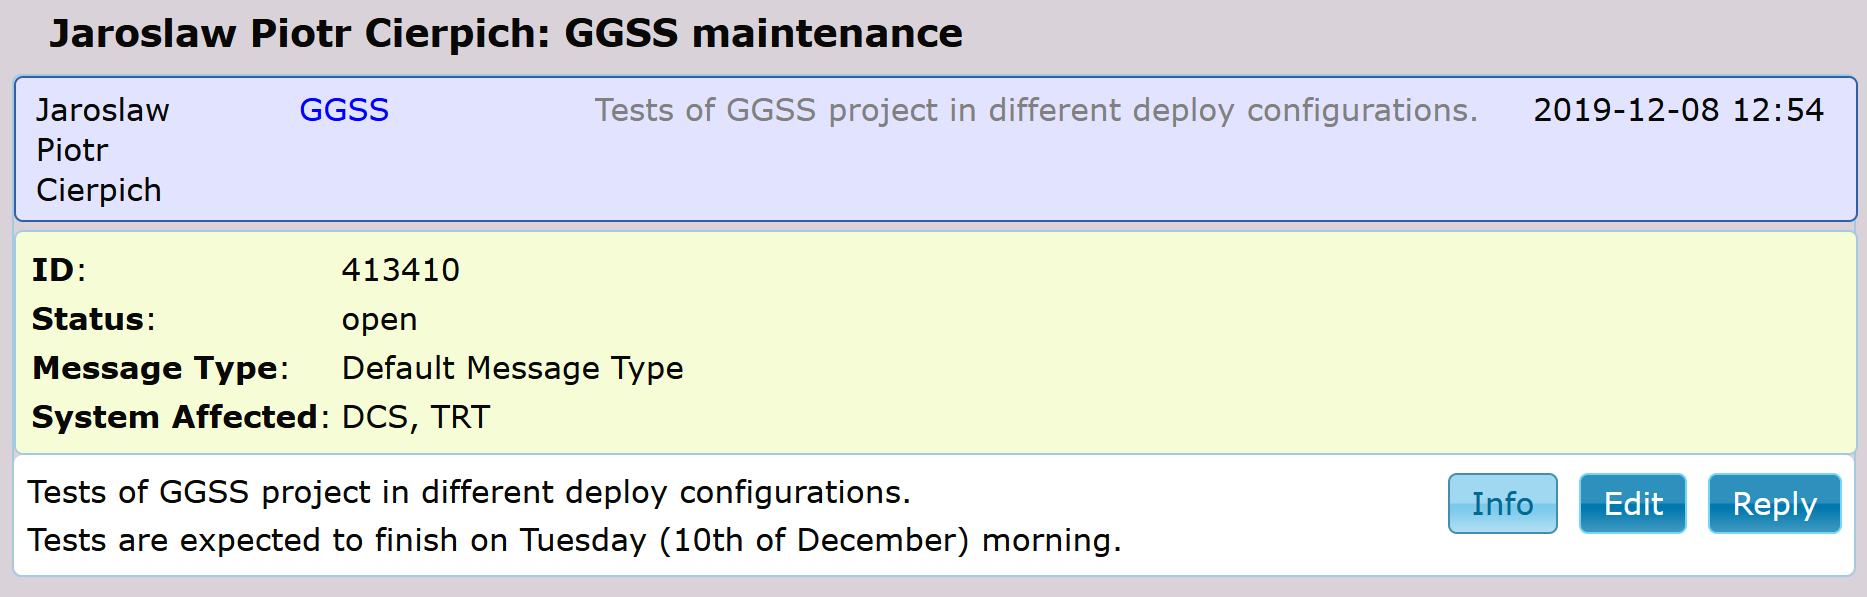
\includegraphics[width=\textwidth]{res/png/elisa}
\end{figure}

Pliki wykonywalne aplikacji \textit{ggssrunner} wygenerowane zostały za pomocą przygotowanego przez autorów środowiska CI/CD. Zostały one umieszczone na komputerze produkcyjnym. Kolejnym krokiem było zalogowanie się do panelu \textit{WinCC OA} służącego do monitorowania działania detektora ATLAS oraz wybranie panelu odpowiedzialnego za dostarczanie informacji o~systemie \gls*{ggss}. 

\begin{figure}[H]
\centering
\caption{Panel WinCC OA monitorujący działanie systemu \gls*{ggss}}
\label{fig:ggss}
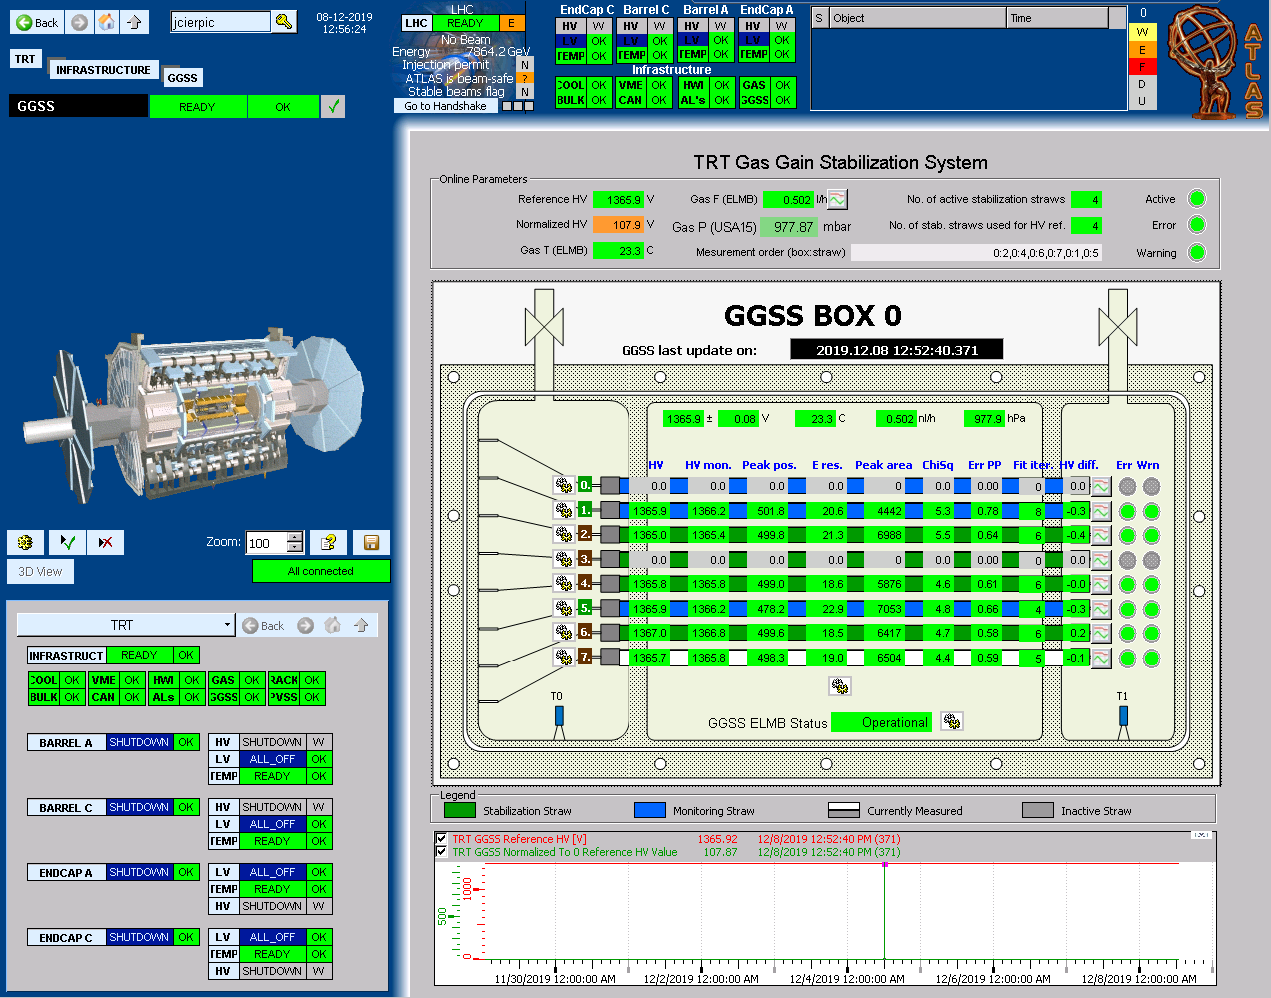
\includegraphics[width=\textwidth]{res/png/ggssStraw}
\end{figure}

\newpage
Następnym etapem było przeprowadzenie procesu wyłączania systemu \gls*{ggss} za pomocą przycisku \textit{Stop} znajdującego się na dedykowanym panelu konfiguracyjnym ukazanym na Rys. \ref{fig:ggsspanel}. 

\begin{figure}[H]
\centering
\caption{Panel konfiguracyjny systemu \gls*{ggss} podczas działania systemu}
\label{fig:ggsspanel}
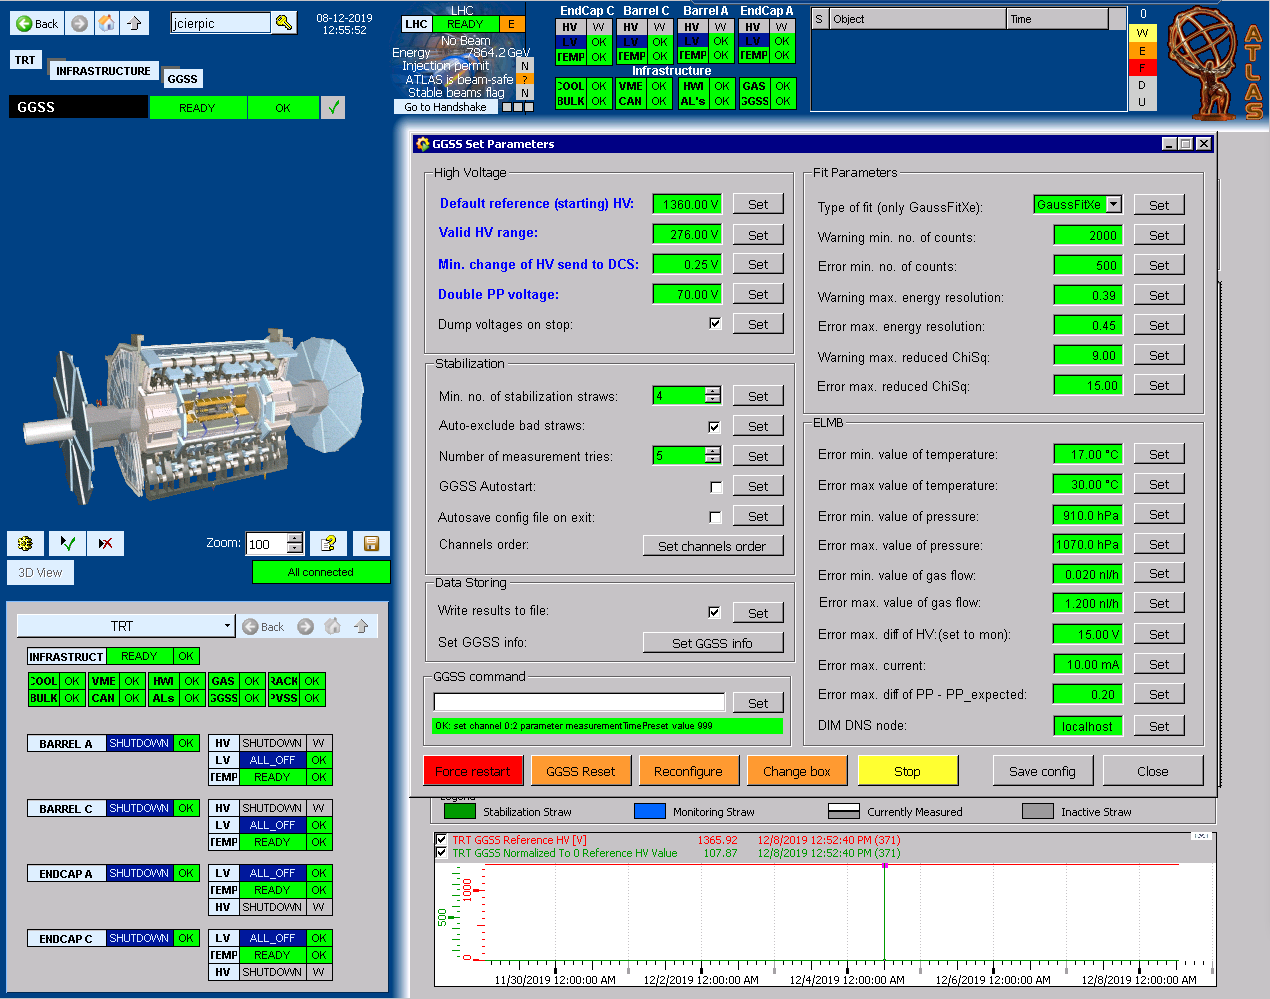
\includegraphics[width=\textwidth]{res/png/ggssConfig}
\end{figure}


\newpage
Po wyłączeniu systemu należało również przerwać działanie poprzedniej wersji aplikacji \textit{ggssrunner} za pomocą skryptu \textit{ggss\_monitor.sh} (listing \ref{lst:ggssstop}). Za pomocą tego skryptu został również potwierdzony stan aplikacji po wyłączeniu.


\begin{lstlisting}[language=Cmd, caption={Zatrzymanie działania aplikacji \textit{ggssrunner}}, label={lst:ggssstop}]
user@host:~$ ./ggss_monitor.sh check
ggssrunner is running.

user@host:~$ ./ggss_monitor.sh stop
ggssrunner: no process found
Creating lock /localdisk/ggss/bin/autostartggss.lock

user@host:~$ ./ggss_monitor.sh check
ggssrunner is NOT running. /localdisk/ggss/bin/autostartggss.lock exists. Remove it or start GGSS manually
\end{lstlisting}



Po wykonaniu wyżej wymienionych czynności podmieniony został plik wykonywalny aplikacji \textit{ggssrunner} na przygotowany przez autorów. Zmiana została wykonana poprzez modyfikacje \textbf{dowiązania symbolicznego}. Następnie aplikacja uruchomiona została ponownie za pomocą skryptu \textit{ggss\_monitor.sh} (listing \ref{lst:ggssstart}) oraz z~poziomu panelu \textit{WinCC OA}. Stan panelu monitorującego system \gls*{ggss} jest widoczny na Rys. \ref{fig:ggssafterstart}.

\begin{lstlisting}[language=Cmd, caption={Ponowne uruchomienie aplikacji \textit{ggssrunner}}, label={lst:ggssstart}]
user@host:~$ ./ggss_monitor.sh remove_lock
Removing lock /localdisk/ggss/bin/autostartggss.lock

user@host:~$ ./ggss_monitor.sh check
ggssrunner is NOT running.

user@host:~$ ./ggss_monitor.sh check_start
\end{lstlisting}

\begin{figure}
\centering
\caption{Panel WinCC OA monitorujący działanie systemu \gls*{ggss} po ponownym uruchomieniu systemu (widoczny w~lewym górnym rogu stan \textit{STARTING})}
\label{fig:ggssafterstart}
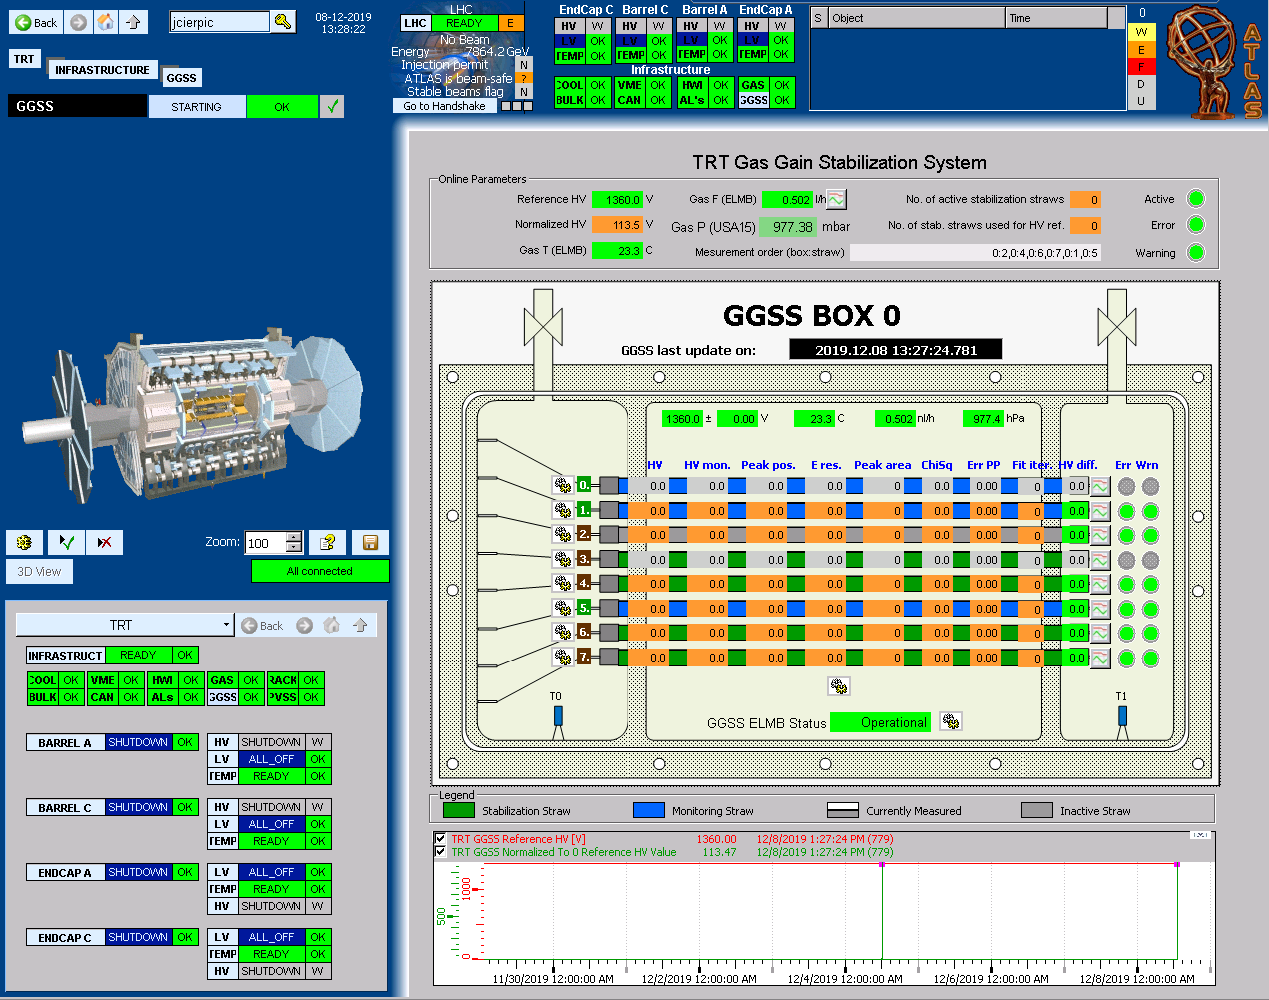
\includegraphics[width=\textwidth]{res/png/ggssPoStarcie}
\end{figure}

\newpage
Dodatkowo użyty został skrypt pozwalający na monitorowanie zużycia zasobów pamięci przez aplikację (listing \ref{lst:ggssmem1}). Sposób użycia oraz fragment generowanego przez ten skrypt wyjścia przedstawia listing \ref{lst:ggssmem2}. 

\begin{lstlisting}[language=bash, caption={Skrypt \textit{check\_mem\_ggssrunner.sh} służacy do monitorowania pamięci używanej przez aplikację \textit{ggssrunner}}, label={lst:ggssmem1}]
#!/bin/bash
while true
do
    ps afux | egrep " ./ggssrunner" | awk -v date="$(date +"%Y.%m.%d %H:%M:%S")" '{print date, $5}'
    sleep 1m
done
\end{lstlisting}


\begin{lstlisting}[language=Cmd, caption={Wywołanie oraz fragment wyjścia skryptu \textit{check\_mem\_ggssrunner.sh} służacego do monitorowania pamięci używanej przez aplikację \textit{ggssrunner}}, label={lst:ggssmem2}]
user@host:~$ ./check_mem_ggssrunner.sh
2019.12.08 15:15:26 638800
2019.12.08 15:16:26 638800
2019.12.08 15:17:26 638800
2019.12.08 15:18:26 638800
2019.12.08 15:19:26 638800
2019.12.08 15:20:27 638800
2019.12.08 15:21:27 638800
2019.12.08 15:22:27 638800
\end{lstlisting}

W takim stanie system pozostawiony został na dłuższy (ponad 6 godzin) czas. Idea testu polegała na sprawdzeniu, czy przez ten czas działanie systemu pozostanie stabilne i~nie pojawią się żadne błędy.

\section{Wyniki testu}
Test każdej z~przygotowanych konfiguracji trwał \textbf{ponad 6 godzin}. Tabela \ref{tab:wyniki} przedstawia rezultaty.

\begin{table}[]
\begin{tabular}{|c|c|c|c|}
\hline
\rowcolor[HTML]{ECF4FF} 
\textbf{\begin{tabular}[c]{@{}c@{}}Konfiguracja \\ (debug/release)\end{tabular}} & \textbf{\begin{tabular}[c]{@{}c@{}}Sposób linkowania \\ biblioteki Boost\end{tabular}} & \textbf{Wygenerowane błędy}                                                              & \textbf{\begin{tabular}[c]{@{}c@{}}Zaalokowana \\ pamięć\end{tabular}} \\ \hline
debug                                                                            & statyczne                                                                              & brak                                                                                     & stała                                                                  \\ \hline
release (-O3)                                                                    & statyczne                                                                              & \begin{tabular}[c]{@{}c@{}}błąd zarejestrowany\\ dla całego systemu \\ GGSS\end{tabular} & stała                                                                  \\ \hline
release (-O2)                                                                    & statyczne                                                                              & brak                                                                                     & stała                                                                  \\ \hline
debug                                                                            & dynamiczne                                                                             & brak                                                                                     & stała                                                                  \\ \hline
release (-O3)                                                                    & dynamiczne                                                                             & \begin{tabular}[c]{@{}c@{}}błąd zarejestrowany\\ dla konkretnej\\ słomki\end{tabular}    & stała                                                                  \\ \hline
\end{tabular}
\caption{Wyniki testów systemu \gls*{ggss} po wprowadzonych zmianach}
\label{tab:wyniki}
\end{table}

Podczas przeprowadzania testów wersji produkcyjnej zostały wykryte błędy w~działaniu, co zostało zakomunikowane na panelu WinCC OA. Błędy te pojawiły się zarówno na poziomie całego systemu (Rys. \ref{fig:ggssErrorScada}) , jak i~pojedynczej słomki (Rys. \ref{fig:ggssErrorStrawScada}). Pojawienie się błędów było skutkiem zastosowania w~czasie kompilacji flagi optymalizacji \textit{-O3}. Jest to domyślna flaga stosowana przez narzędzie \gls*{cmake} dla wersji produkcyjnej. Podczas kompilacji aplikacji \textit{ggssrunner} w~takiej konfiguracji widoczne były dwa ostrzeżenia, zatem błędy nie były dla autorów zaskoczeniem. Flaga \textit{-O3} oznacza agresywną politykę optymalizacji, co często prowadzi do zmiany zachowania aplikacji. Została więc wprowadzona zmiana w~sposobie kompilacji aplikacji w~wersji produkcyjnej - flaga ta została zastąpiona przez jej łagodniejszy i~stabilniejszy odpowiednik \textit{-O2}, powszechnie wykorzystywany do tworzenia wersji produkcyjnych oprogramowania. Testy wykonane z~użyciem tej flagi nie wyprodukowały żadnych błędów. 

Testy wersji deweloperskiej (w obu konfiguracjach) odbyły się bez problemów - nie zostały wygenerowane żadne błędy ani ostrzeżenia. 

W każdym z~przypadków ilość zaalokowanej przez program pamięci pozostawała stała przez cały czas trwania testu. Oznacza to brak znaczących problemów z~zarządzaniem pamięcią (takich jak wycieki pamięci).

Wyniki przeprowadzonych testów stanowią potwierdzenie poprawności wprowadzonych przez autorów zmian w~systemie. 

\begin{figure}
\centering
\caption{Błąd w~działaniu aplikacji \textit{ggssrunner} na poziomie całego systemu widoczny w~panelu WinCC OA (czerwone koło w~prawym górnym rogu panelu \gls*{ggss})}
\label{fig:ggssErrorScada}
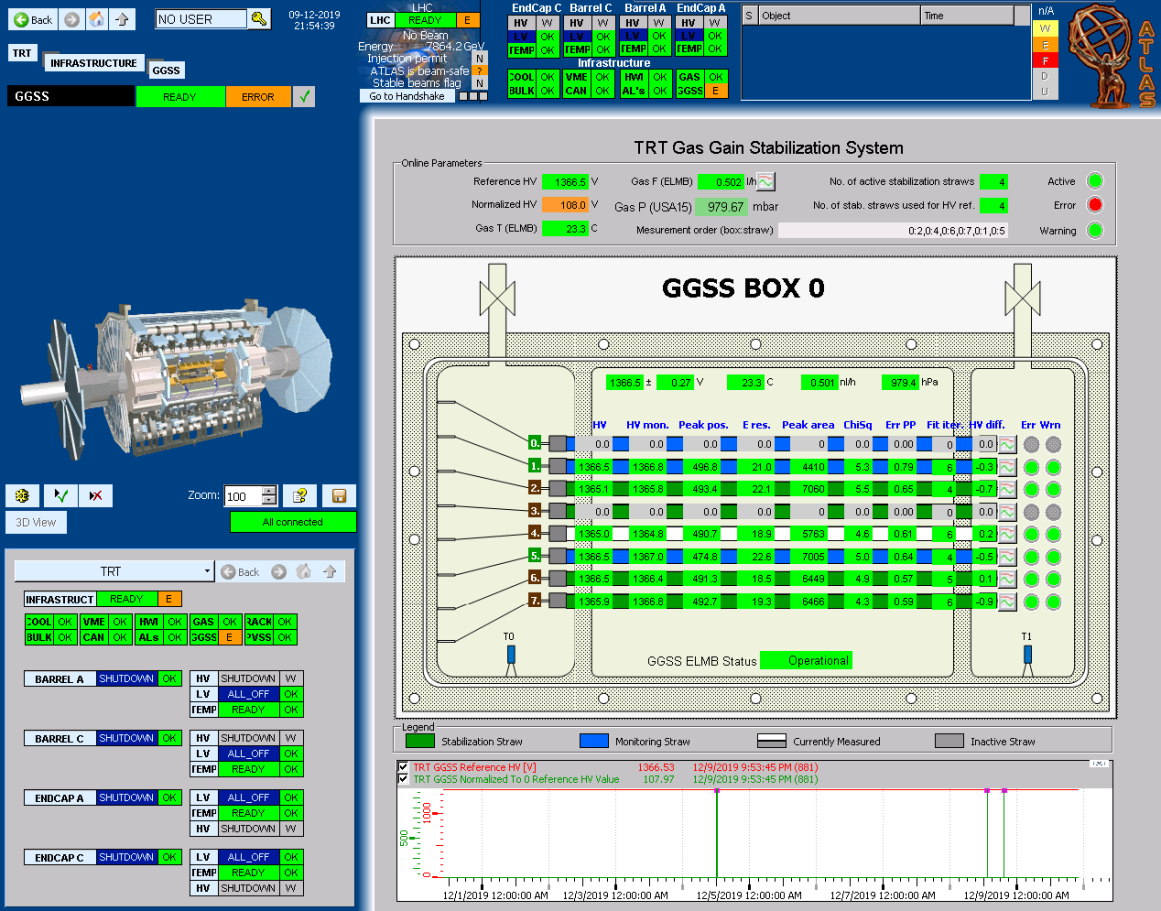
\includegraphics[width=\textwidth]{res/png/ggssError}
\end{figure}


\begin{figure}
\centering
\caption{Błąd w~działaniu aplikacji \textit{ggssrunner} na poziomie pojedynczej słomki widoczny w~panelu WinCC OA (czerwone koło obok drugiej słomki)}
\label{fig:ggssErrorStrawScada}
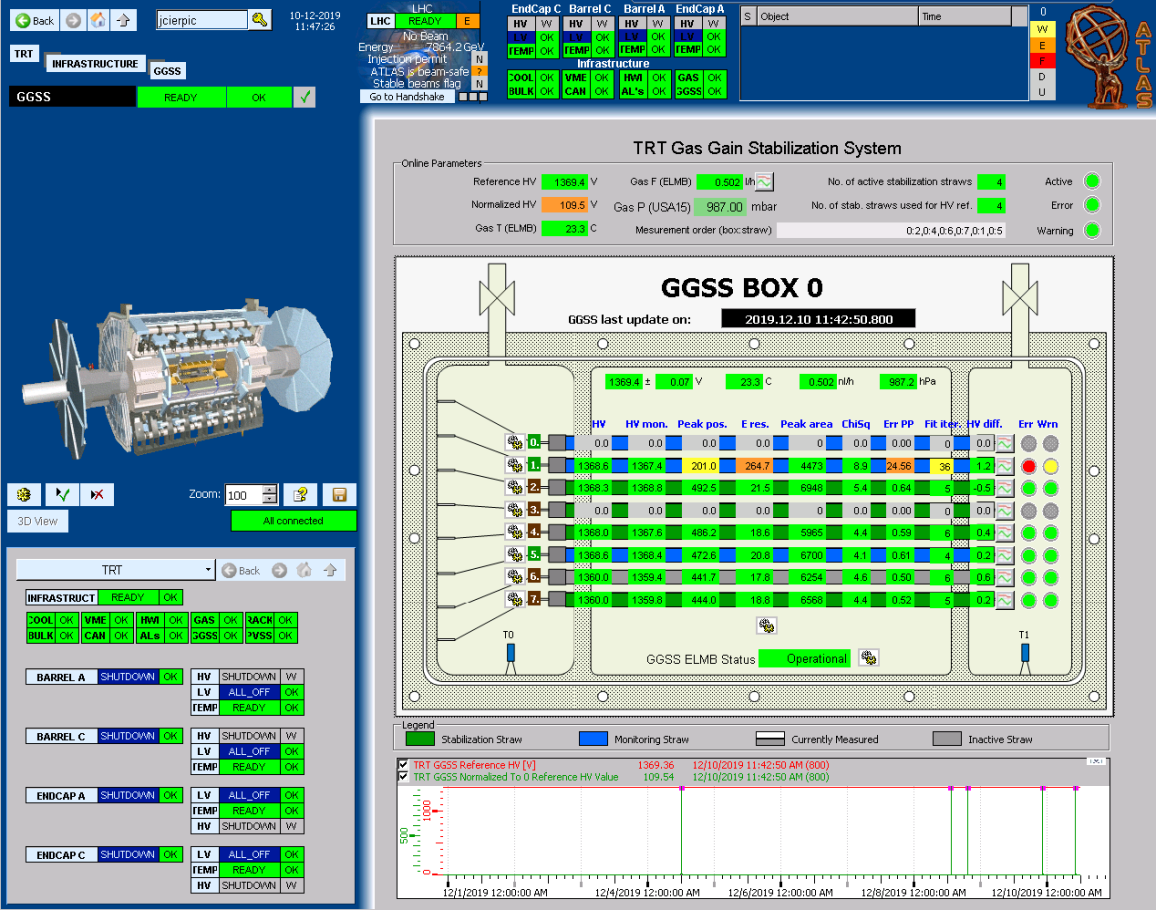
\includegraphics[width=\textwidth]{res/png/errStraw}
\end{figure}
